\section{Observability med Prometheus og Grafana}

For å overvåke VideoAPI-ets oppførsel i drift ble det implementert støtte for helsesjekker, Prometheus-metrikker og Grafana-dashboards. Formålet var å gjøre avvik og feil synlige uten å måtte analysere containerlogger. API-et eksponerer derfor informasjon om tre områder: prosessens helsetilstand, tilgjengeligheten til AntMedia og NHN, samt utviklingen av trafikk, feil, autentisering og rate limiting over tid.

Løsningen er bygget rundt \texttt{prometheus-net}. I request-pipelinen brukes \texttt{UseHttpMetrics()} for automatisk innsamling av HTTP-metrikker, mens \texttt{MapMetrics()} eksponerer metrikker på \texttt{/metrics}. Prometheus kan dermed hente data fra API-et med faste intervaller, uten at API-et selv trenger å sende ut data.

\begin{lstlisting}[
    language={[Sharp]C},
    label=lst:observability-pipeline,
    caption={Registrering av Prometheus-metrikker i request-pipelinen}
]
app.UseHttpMetrics();
app.MapControllers();
app.MapMetrics();
app.MapVideoHealthChecks();
\end{lstlisting}

\subsection{Helsesjekker}

API-et eksponerer to helsesjekk-endepunkter. \texttt{/health/live} verifiserer kun om API-prosessen kjører, uten å utføre kall mot AntMedia eller NHN, og fungerer dermed som en liveness check for containeren. \texttt{/health/ready} verifiserer derimot om API-et er klart til å håndtere trafikk. Denne sjekken benytter dedikerte health checks for AntMedia og NHN, og kaller \texttt{IsAvailableAsync()} på hver provider.

\begin{lstlisting}[
    language={[Sharp]C},
    label=lst:healthcheck-registration,
    caption={Registrering av readiness-sjekker for AntMedia og NHN}
]
healthChecks
    .AddCheck<AntMediaHealthCheck>("antmedia", tags: ["ready"])
    .AddCheck<NHNHealthCheck>("nhn", tags: ["ready"]);
\end{lstlisting}

Health check-resultatene videresendes også til Prometheus via \texttt{ForwardToPrometheus()}. Dette gjør det mulig for Grafana å presentere provider-status som måleverdier. Verdien \texttt{2} indikerer healthy, \texttt{1} degraded og \texttt{0} unhealthy. Den samme informasjonen kan dermed leses direkte fra API-et og visualiseres historisk i Grafana.

\subsection{Egne metrikker i API-et}

I tillegg til de innebygde HTTP-metrikkene ble det implementert egendefinerte metrikker i \texttt{VideoMetrics}. Disse måler VideoAPI-spesifikke hendelser som aktive rom per provider, antall feil per exception-type, Keycloak-tokenkall og rate limit-avvisninger. \texttt{VideoMetrics} registreres som en singleton bak grensesnittet \texttt{IVideoMetrics}, slik at controllere og middleware kan registrere hendelser uten direkte kobling til Prometheus.

\begin{lstlisting}[
    language={[Sharp]C},
    label=lst:custom-metrics,
    caption={Egne Prometheus-metrikker for VideoAPI-et}
]
private static readonly Gauge _activeRooms =
    Prometheus.Metrics.CreateGauge(
        "hdo_active_rooms_total",
        "Number of active video rooms per provider.",
        labelNames: ["provider"]
    );

private static readonly Counter _errors =
    Prometheus.Metrics.CreateCounter(
        "hdo_errors_total",
        "Total number of unhandled exceptions, labelled by exception type.",
        labelNames: ["exception_type"]
    );
\end{lstlisting}

Romtellerne oppdateres i \texttt{RoomsController}. Ved opprettelse av et rom inkrementeres telleren for valgt provider, mens den dekrementeres ved sletting. Telleren gir ikke en full historisk oversikt etter restart, ettersom den lever i API-prosessen, men er nyttig for å overvåke aktivitet mens systemet kjører.

\begin{lstlisting}[
    language={[Sharp]C},
    label=lst:room-metrics,
    caption={Oppdatering av rommeteller ved opprettelse og sletting}
]
metrics.RoomCreated(providerKey);

...

metrics.RoomDeleted(providerKey);
\end{lstlisting}

Feil registreres i \texttt{GlobalExceptionHandler}. Når en exception håndteres, logges typen i \texttt{hdo\_errors\_total}, noe som muliggjør skille mellom for eksempel \texttt{ArgumentException}, \texttt{ExternalServiceException}, \texttt{NotFoundException} og \texttt{NotSupportedException} i Grafana. Rate limiting måles i \texttt{RateLimitingExtensions}, der avviste kall klassifiseres som enten \texttt{global} eller \texttt{auth}.

\subsection{Prometheus}

Prometheus kjøres som en egen container i Docker Compose og henter metrikker fra API-et hvert 15. sekund via \texttt{/metrics}. Siden containerne ligger på samme Docker-nettverk, benytter Prometheus servicenavnet \texttt{hdo-videoapi} i stedet for en ekstern URL. Scrape-trafikken foregår dermed internt mellom containerne.

\begin{lstlisting}[
    language={},
    label=lst:prometheus-config,
    caption={Prometheus-konfigurasjon for scraping av VideoAPI}
]
global:
  scrape_interval: 15s

scrape_configs:
  - job_name: 'hdo-videoapi'
    scheme: http
    static_configs:
      - targets: ['hdo-videoapi:8080']
    metrics_path: /metrics
\end{lstlisting}

Compose-oppsettet starter Prometheus først når API-containeren er rapportert som healthy. Metrikkdata lagres i Docker-volumet \texttt{prometheus\_data}, slik at data persisteres mellom normale restarter. Data går kun tapt dersom volumet slettes, for eksempel ved bruk av \texttt{docker compose down -v}.

\subsection{Grafana}

Grafana brukes som visualiseringslag over Prometheus. Datakilden provisioneres automatisk via \url{grafana-provisioning/datasources/prometheus.yml} og peker til \url{http://prometheus:9090}. Dette eliminerer behovet for manuell konfigurering av Prometheus i Grafana etter første oppstart.

\begin{lstlisting}[
    language={},
    label=lst:grafana-datasource,
    caption={Automatisk konfigurering av Prometheus som Grafana-datasource}
]
apiVersion: 2
datasources:
  - name: Prometheus
    type: prometheus
    uid: PBFA97CFB590B2093
    url: http://prometheus:9090
    isDefault: true
\end{lstlisting}

Det ble utviklet tre dashboards i Grafana. Overview-dashboardet, vist i figur~\ref{fig:grafana-overview}, gir et overordnet bilde av systemtilstanden med providerstatus, aktive rom, request rate og \texttt{5xx}-feil. Provider Health-dashboardet, vist i figur~\ref{fig:grafana-provider-health}, går mer i dybden på AntMedia og NHN hver for seg. Her kan man observere om en provider er nede, om responstiden øker, og hvordan rommene fordeler seg mellom providerne. Security-dashboardet, vist i figur~\ref{fig:grafana-security}, samler målinger knyttet til autentisering og tilgangskontroll, inkludert Keycloak-tokenkall, rate limit-avvisninger og exceptions.

\begin{figure}[htbp]
    \centering
    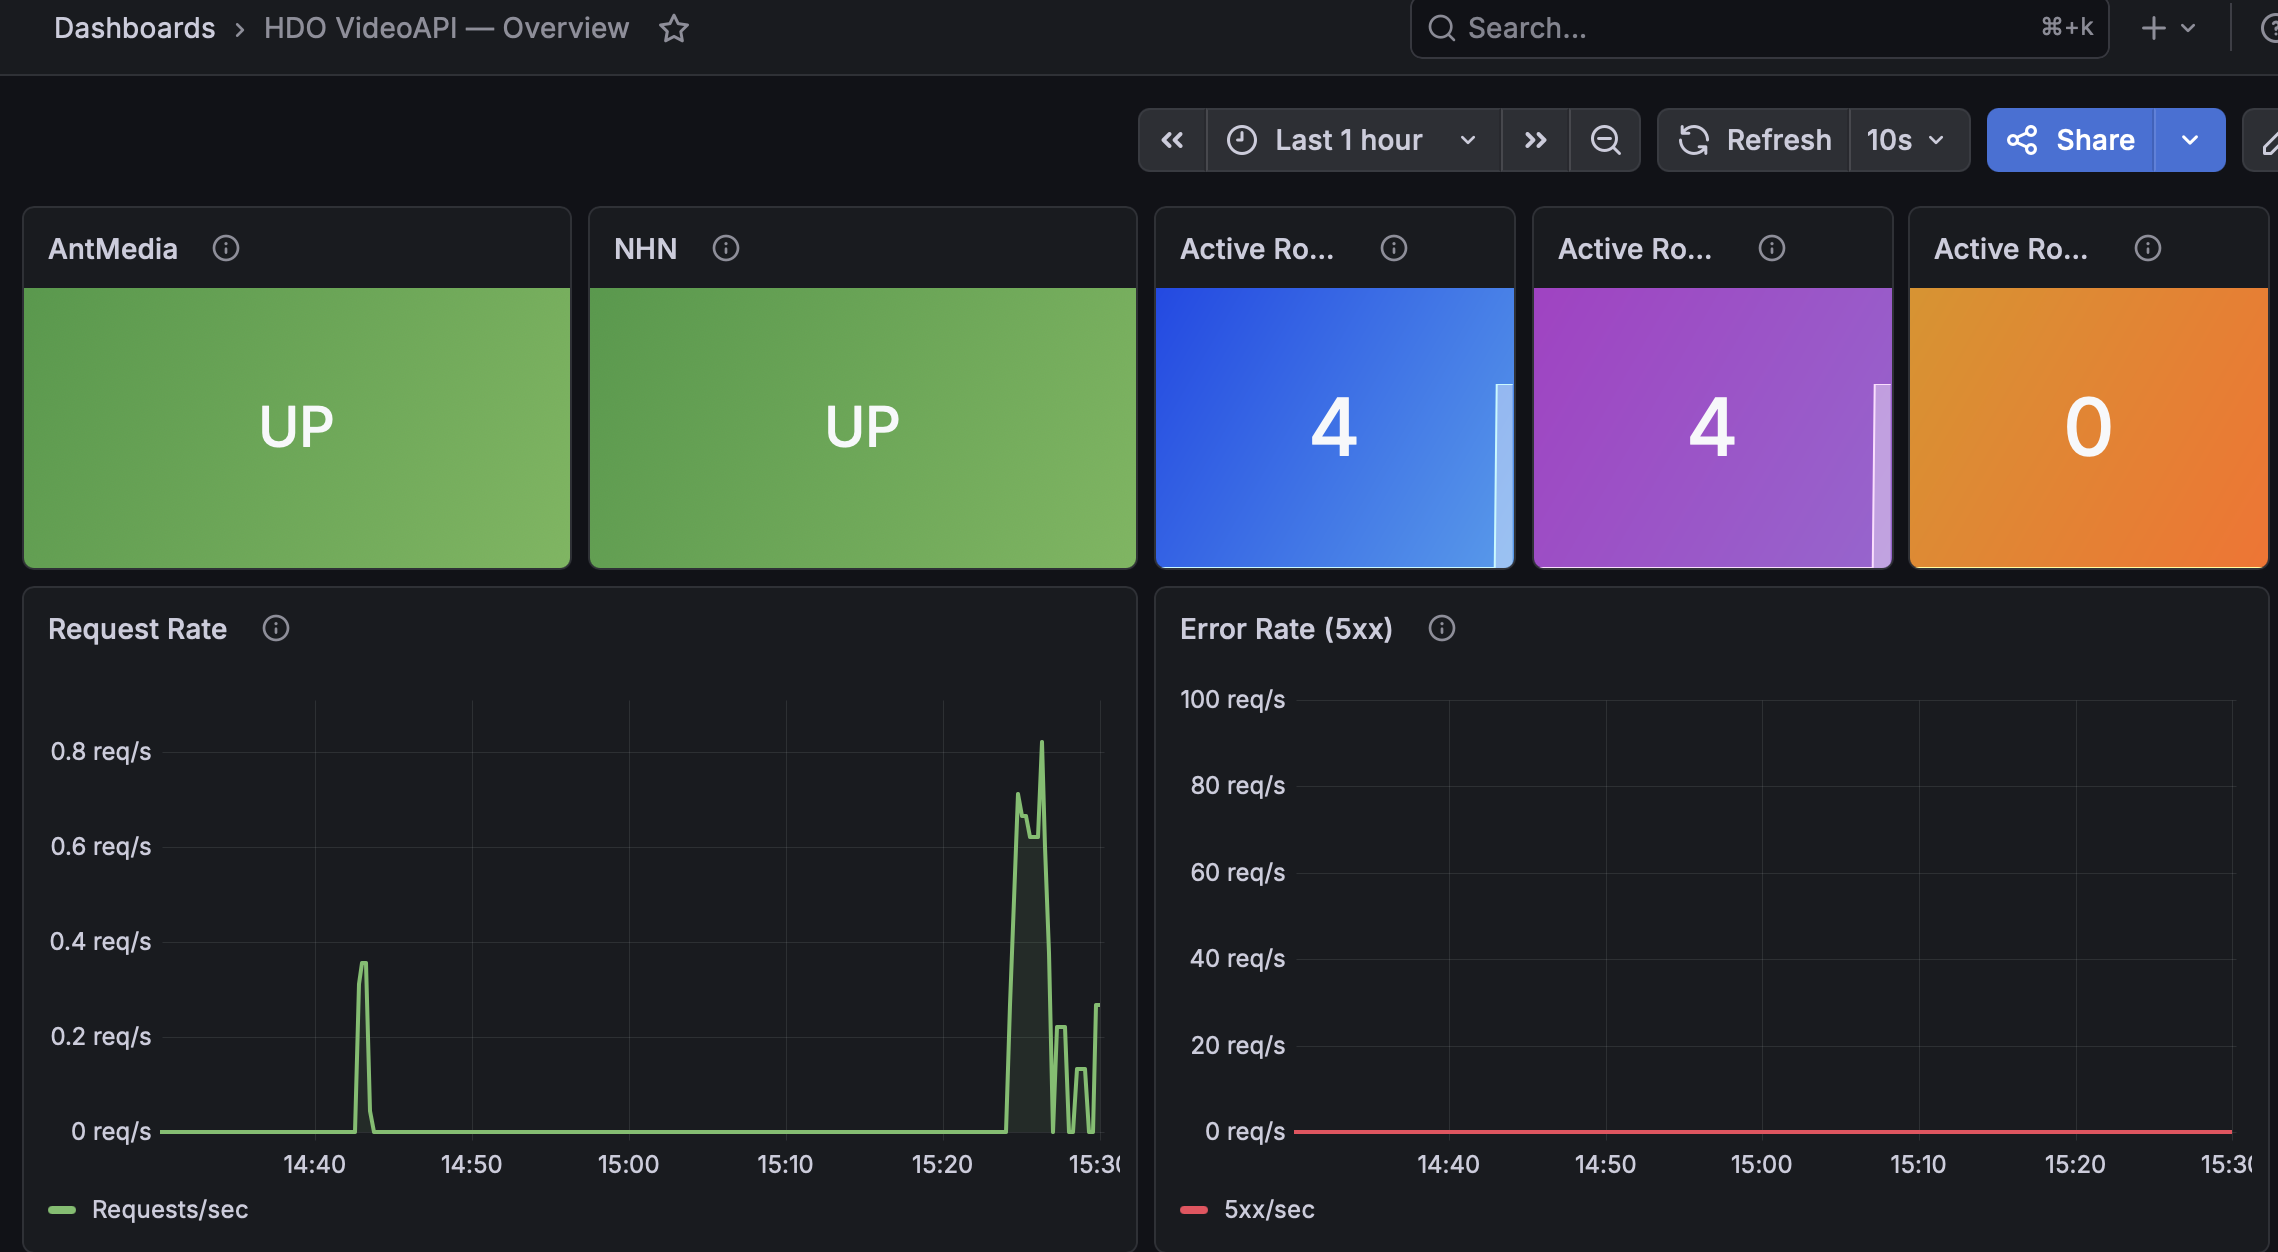
\includegraphics[width=\textwidth]{figures/grafana-overview.png}
    \caption{Overview-dashboardet viser status og informasjon for AntMedia og NHN.}
    \label{fig:grafana-overview}
\end{figure}

\begin{figure}[htbp]
    \centering
    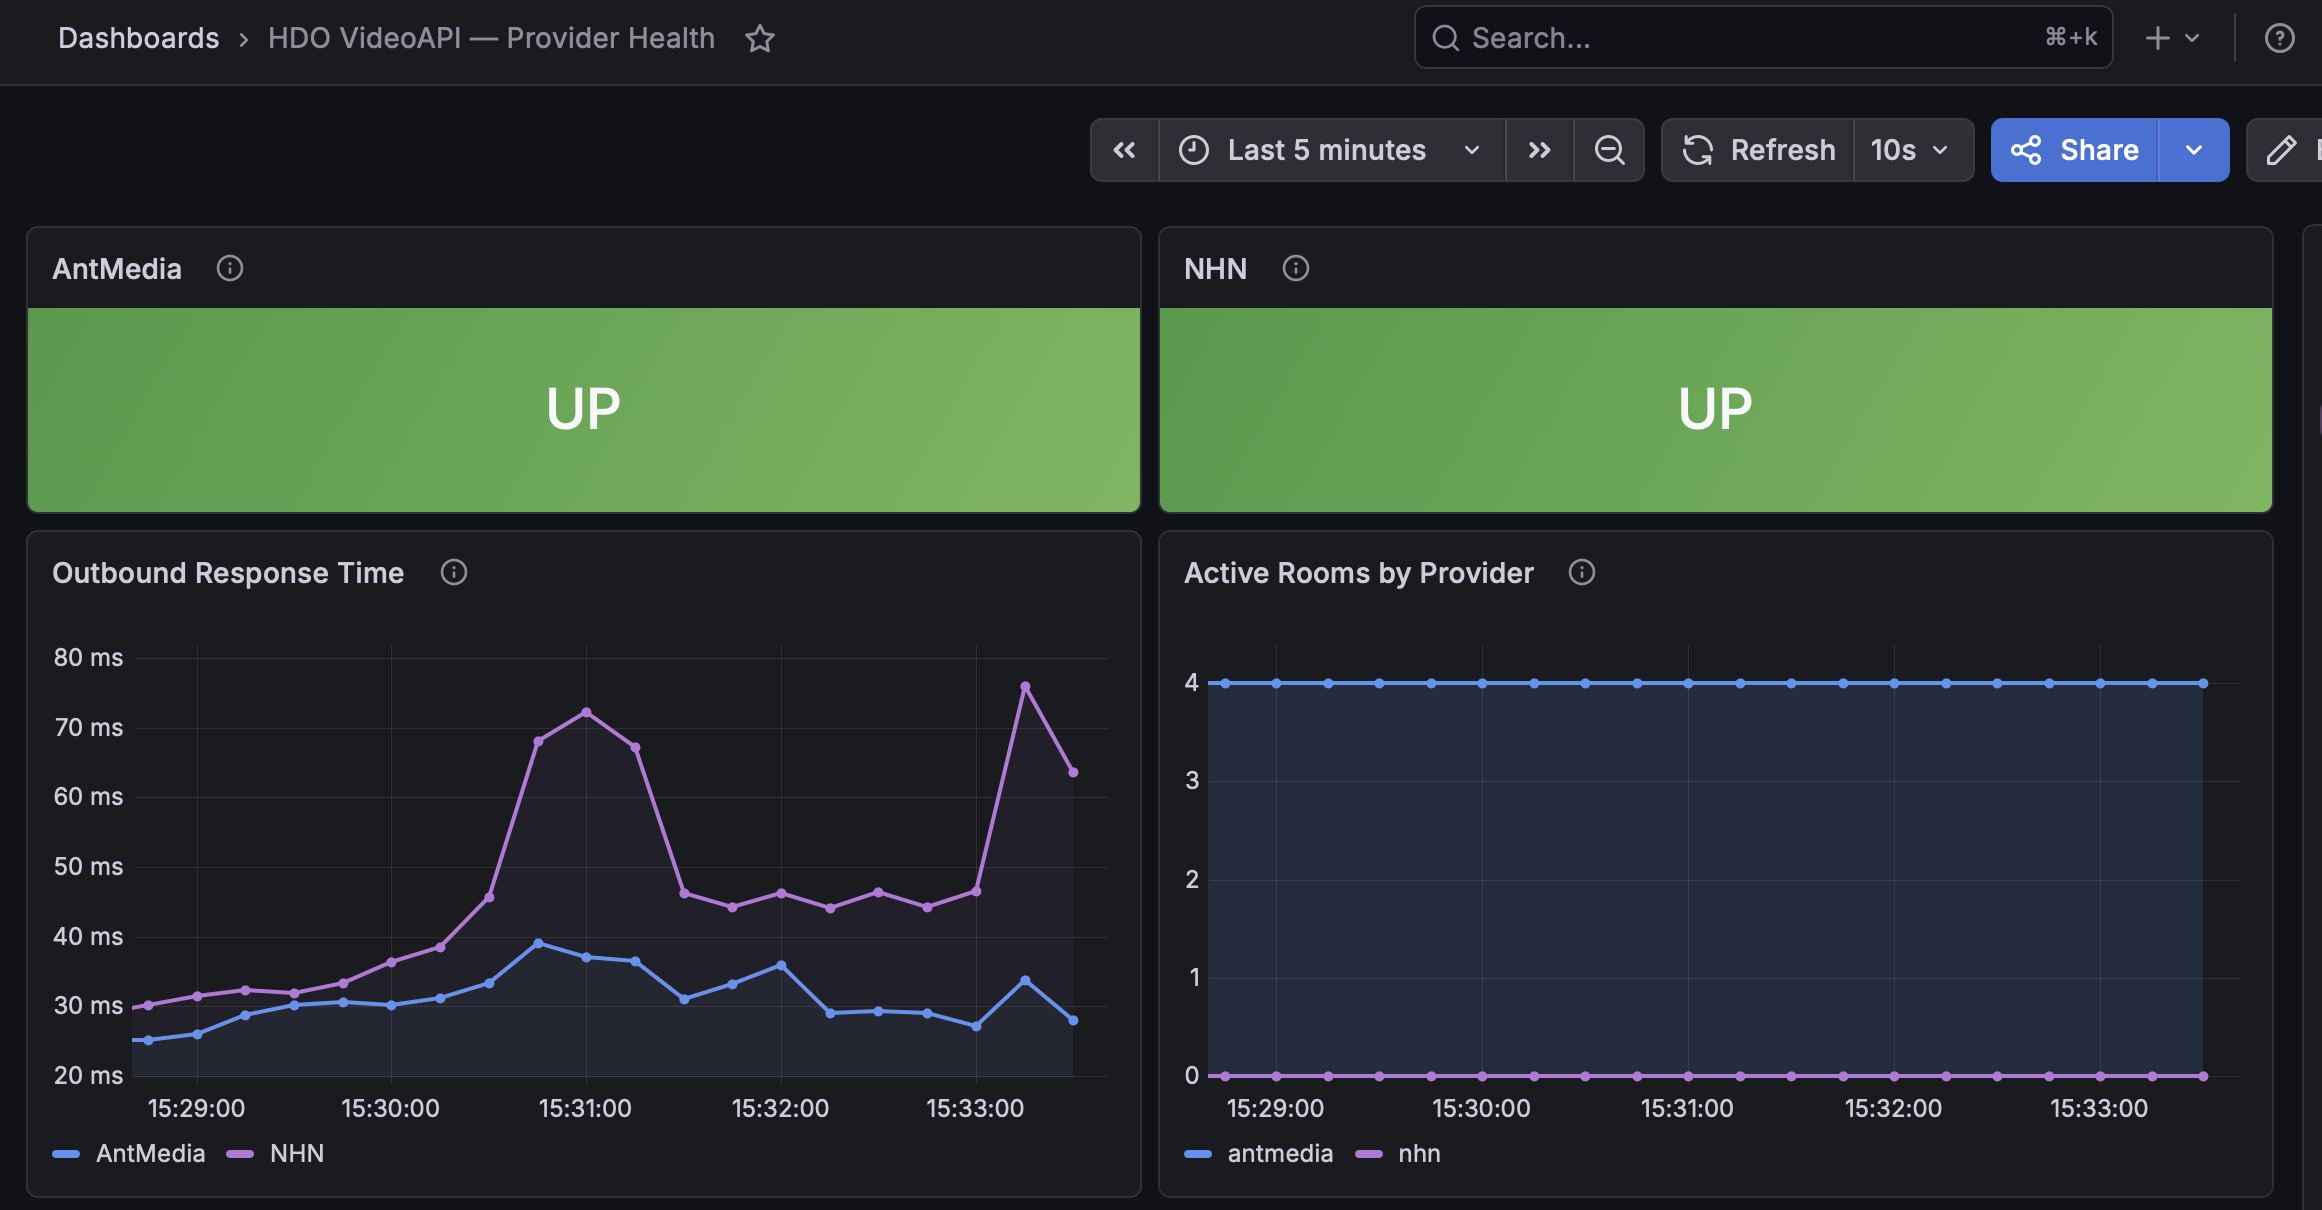
\includegraphics[width=\textwidth]{figures/grafana-provider-health.png}
    \caption{Provider Health-dashboardet viser helsestatus for AntMedia og NHN, responstid mot eksterne providere og aktive rom per provider.}
    \label{fig:grafana-provider-health}
\end{figure}

\begin{figure}[htbp]
    \centering
    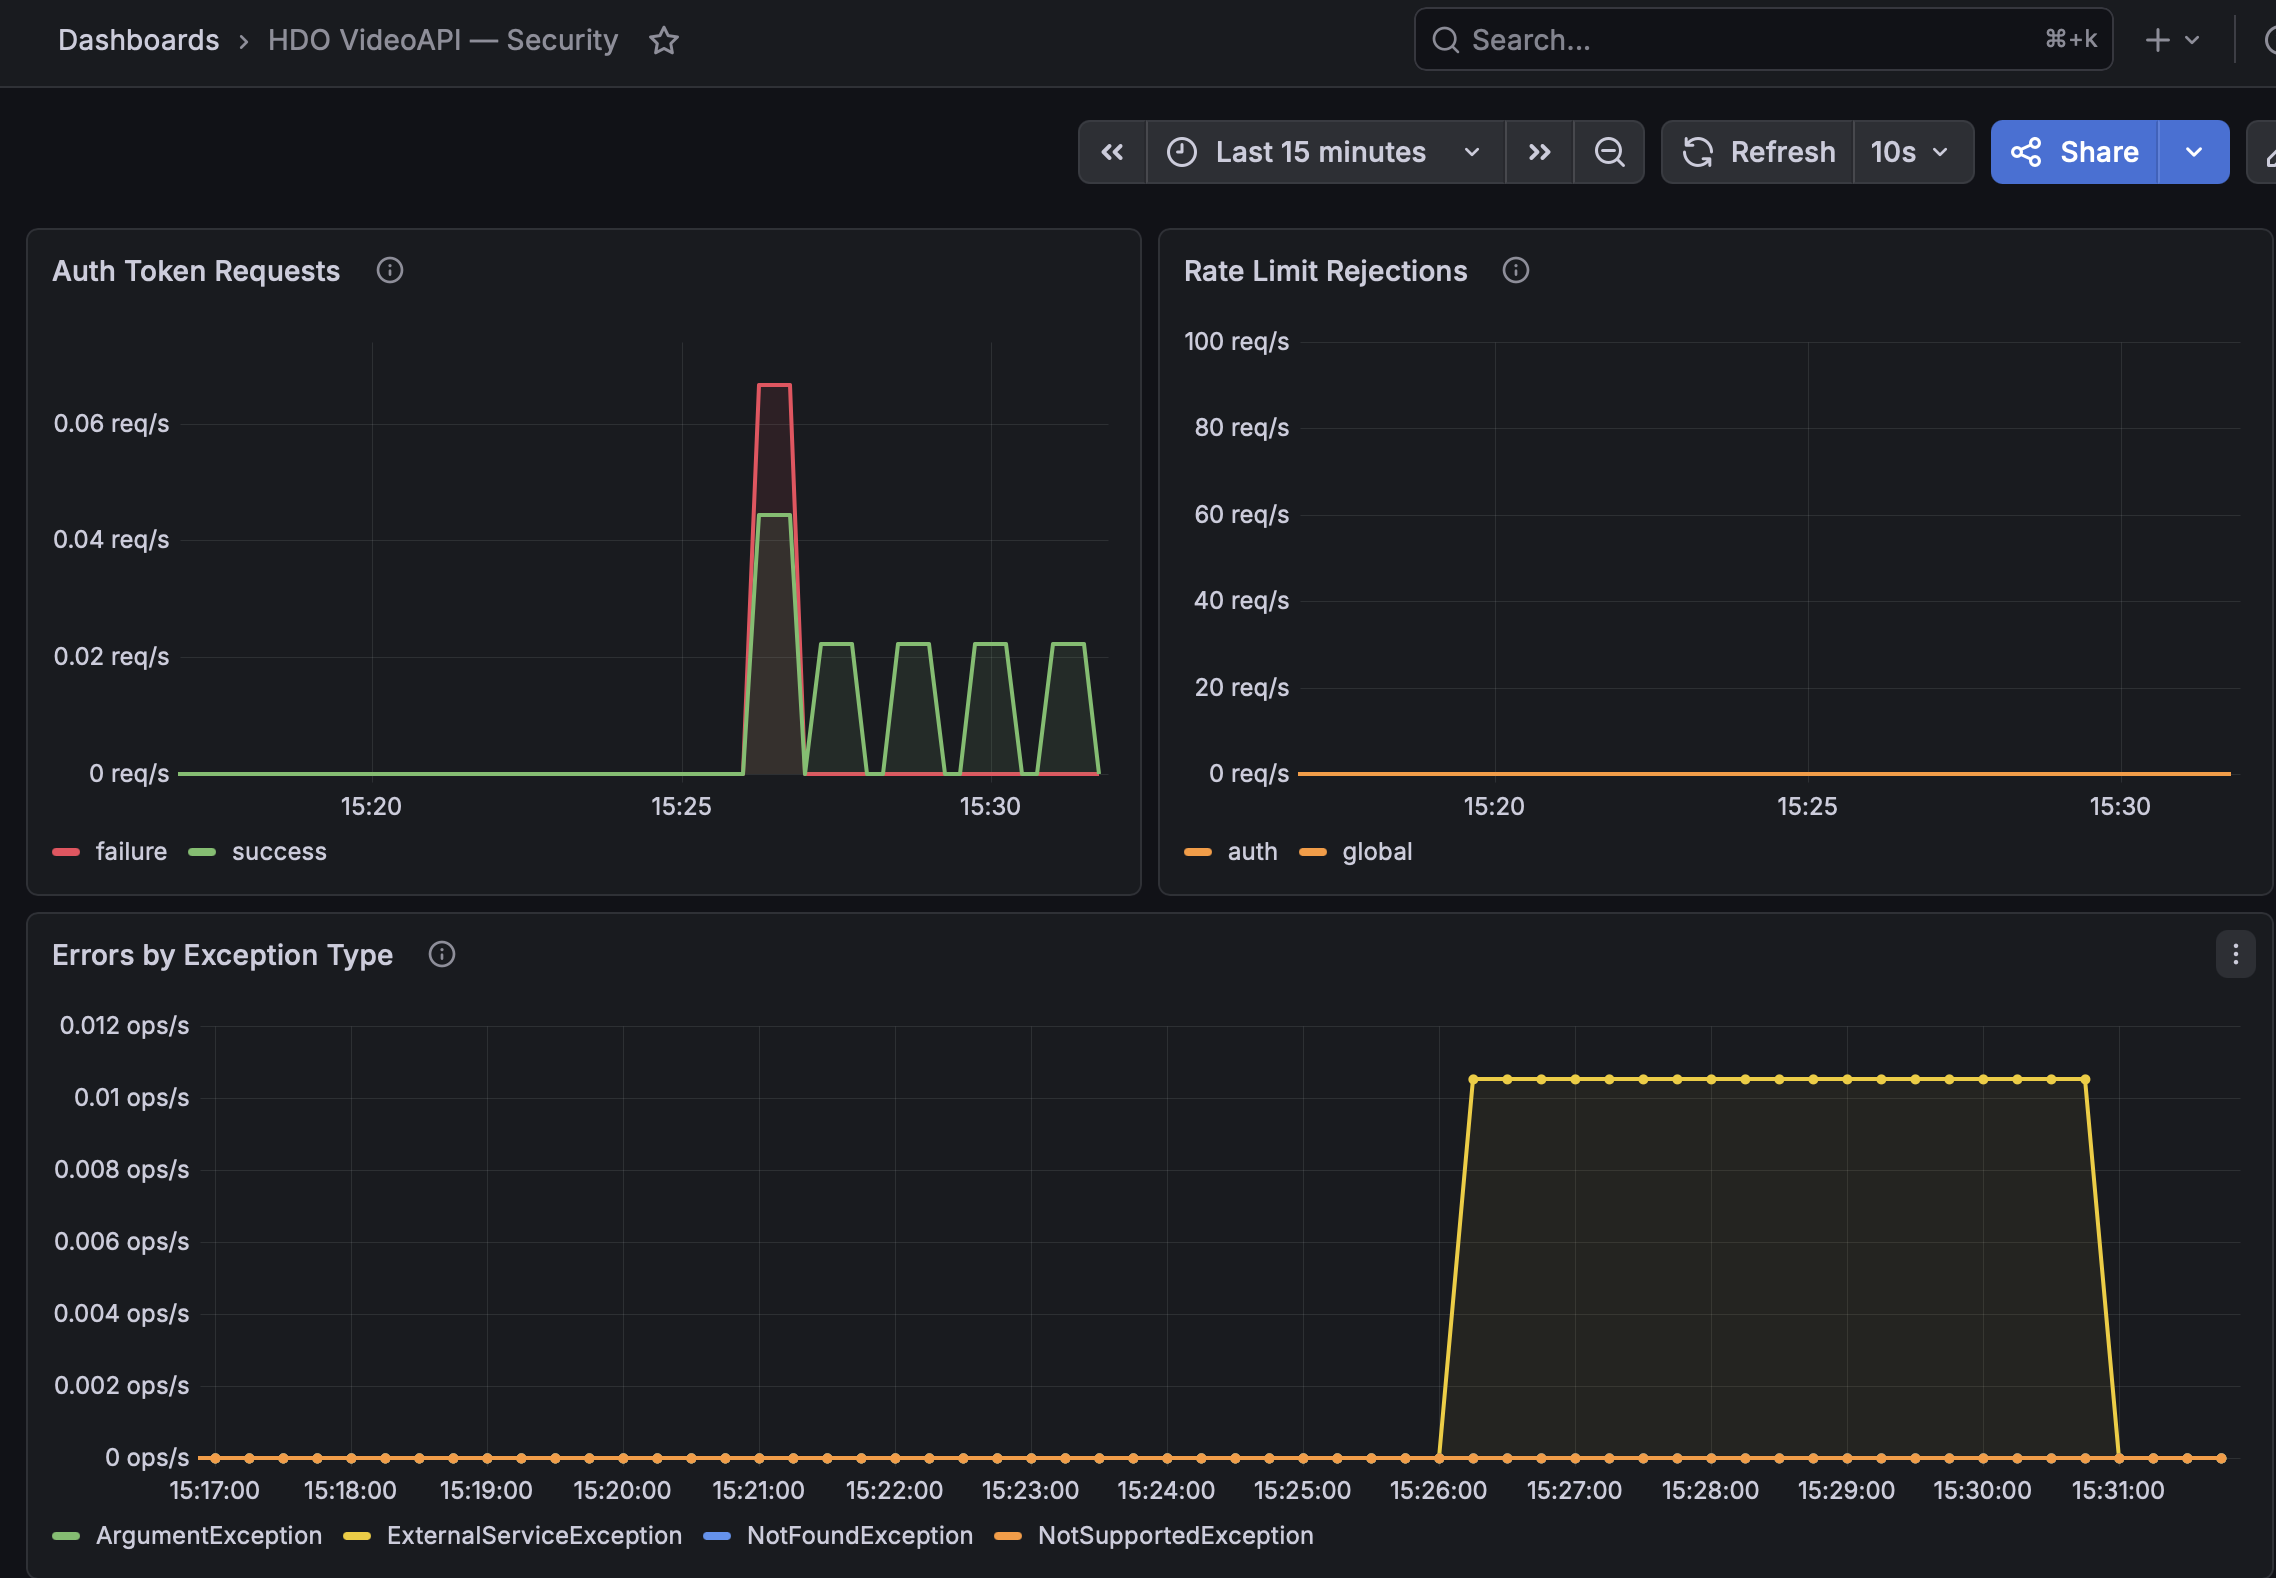
\includegraphics[width=\textwidth]{figures/grafana-security.png}
    \caption{Security-dashboardet viser tokenforespørsler, rate limit-avvisninger og feil fordelt på exception-typer.}
    \label{fig:grafana-security}
\end{figure}

\newpage

Dashboardene kan også aksesseres direkte i nettleseren via \url{http://video-backend.hdolab.no:3000/dashboards}
. Innloggingsinformasjon deles separat med veileder og sensor.

\subsection{Docker Compose-oppsett}

Hele observability-stacken kjøres sammen med API-et i Docker Compose. API-et eksponerer port 80 og 443 på hosten, mens Prometheus og Grafana eksponeres på henholdsvis port 9090 og 3000. Prometheus starter først når API-et rapporteres som healthy, og Grafana starter først når Prometheus er tilgjengelig.

\begin{lstlisting}[
    language={},
    label=lst:compose-observability,
    caption={Prometheus og Grafana i Docker Compose}
]
prometheus:
  image: prom/prometheus:latest
  restart: unless-stopped
  ports:
    - "9090:9090"
  volumes:
    - ./prometheus.yml:/etc/prometheus/prometheus.yml
    - prometheus_data:/prometheus
  depends_on:
    hdo-videoapi:
      condition: service_healthy

grafana:
  image: grafana/grafana:latest
  restart: unless-stopped
  ports:
    - "3000:3000"
  volumes:
    - grafana_data:/var/lib/grafana
    - ./grafana-provisioning:/etc/grafana/provisioning
\end{lstlisting}

Dette ga en enkel driftsmodell. API-et publiserer helsestatus og metrikker, Prometheus henter og lagrer dem, og Grafana visualiserer dem i ferdige dashboards. Løsningen erstatter ikke logging, men gjør det enklere å oppdage feil tidlig og identifisere hvilken del av systemet som feiler.